\newpage
\section{Agile Development(敏捷开发)}
\subsection{What is Agility}
\begin{itemize}
    \item Effective response to change
    \item Drawing the customer onto the team(让用户参与开发)
    \item Rapid, incremental delivery of software(快速增量式交付)
\end{itemize}

\subsection{Agility and the Cost of Change}
\begin{figure}[!htb]
    \centering
    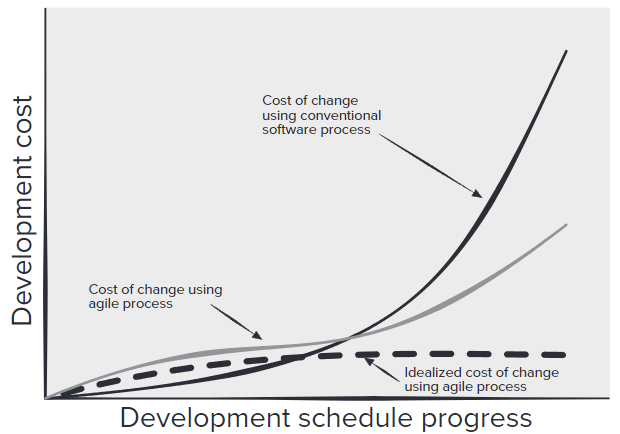
\includegraphics[width=0.309\textwidth]{pic/SE3/Change costs as a function of time in development}
    \caption{Change costs as a function of time in development}
\end{figure}

\subsection{Agility Process}

\subsubsection{Agility Principles}
\begin{itemize}
    \item 频繁开会(开完后开摆)
    \begin{enumerate}
        \item 客户至上
        \item 客户可能不要开发好的代码
        \item 增量式交付
        \item 与用户一起开发
        \item 打鸡血
        \item 当面沟通(即时沟通)
    \end{enumerate}
    \item 不停改进
    \begin{enumerate}
        \setcounter{enumi}{6}
        \item 周期性改进
    \end{enumerate}
\end{itemize}

\subsection{Agile Frameworks}

\subsubsection{Agile Unified Process}

\subsubsection{Extreme Programming(XP)}

\subsubsection{Scrum}
$\left(\enspace{}^{\circ}\;\forall\;{}_{\circ}\enspace\right)$

\begin{figure}[!htb]
    \centering
    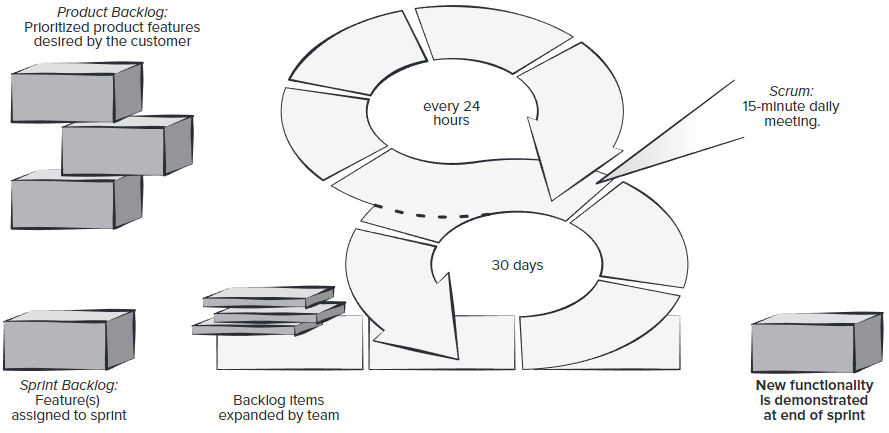
\includegraphics[width=0.42\textwidth]{pic/SE3/Scrum process flow}
    \caption{Scrum process flow}
\end{figure}

\subsubsection{DSDM}

\newpage
\section{Human Aspects of Software Engineering}
\subsection{Characteristics of a Software Engineer}

\subsection{The Psycholog of Software Engineering}

\subsection{The Software Team}

Avoid Team ``Toxicity'':
\begin{itemize}
    \item 工作氛围不融洽(内部勾心斗角)
    \item 高度挫败感(leader 不强)
    \item ``fragmented or poorly coordinated procedures''(程序分散或协调不力)
    \item Unclear definition
    \item 经常失败(leader 不强)
\end{itemize}

\subsection{Team Structures}

\subsection{Agile Team}